\documentclass[11pt]{standalone}
\usepackage{amssymb}
\usepackage{amsmath}
\usepackage[no-math]{fontspec}
\usepackage{unicode-math}
\usepackage{libertinus}
\usepackage{pgf,xcolor}
\usepackage{tikz}
\usetikzlibrary{arrows.meta, backgrounds}
\usepackage{pgfplots}
\pgfplotsset{compat=newest}

\definecolor{my_darkgray}{HTML}{484949}
\definecolor{my_lightgray}{HTML}{F3F4F4}
\definecolor{my_darkblue}{HTML}{005A94}
\definecolor{my_lightblue}{HTML}{CCDEE9}
\definecolor{my_yellow}{HTML}{FFEC7F}
\definecolor{my_red}{HTML}{E60000}
\definecolor{my_orange}{HTML}{E87846}

\begin{document}
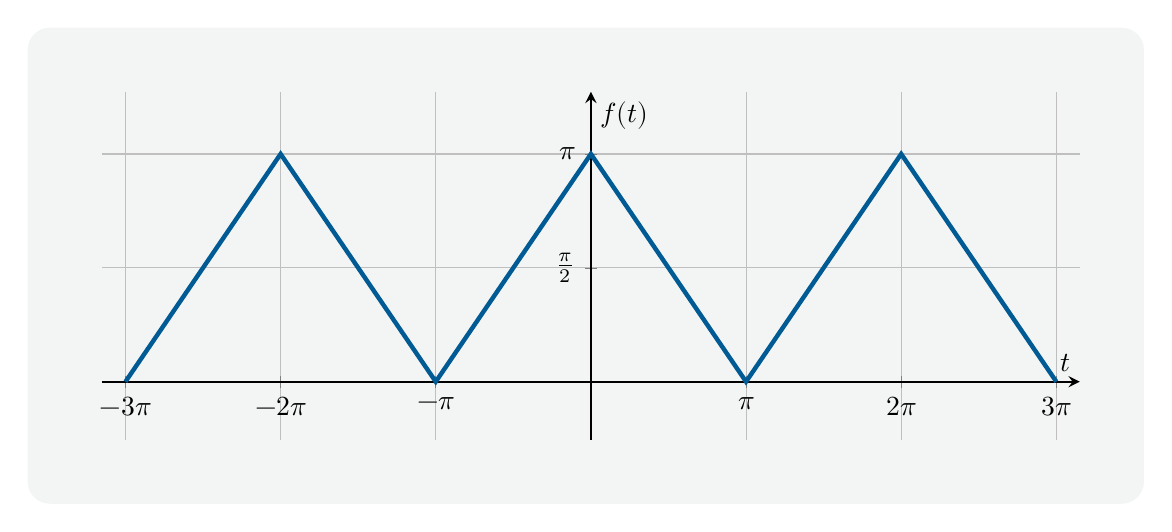
\begin{tikzpicture}[
    show background rectangle,
    background rectangle/.style={fill=my_lightgray, rounded corners=8pt},
    inner frame sep=0.8cm
]
\begin{axis}[
    axis lines = center,
    xlabel = {$t$},
    ylabel = {$f(t)$},
    grid = both,
    % axis equal hier bewusst weggelassen: Bei gleicher Skalierung ueber drei
    % Perioden wird die Abbildung sehr flach; ein festes Seitenverhaeltnis
    % macht den Verlauf besser lesbar.
    axis line style={thick},
    width=14cm, height=6cm,
    xmin=-9.9, xmax=9.9,
    ymin=-0.8, ymax=4.0,
    xtick={-9.42478, -6.28319, -3.14159, 0, 3.14159, 6.28319, 9.42478},
    xticklabels={$-3\pi$, $-2\pi$, $-\pi$, $0$, $\pi$, $2\pi$, $3\pi$},
    ytick={1.5708, 3.14159},
    yticklabels={$\tfrac{\pi}{2}$, $\pi$},
]
% Dreiecksschwingung mit Periode T = 2*pi:
% Spitzen (Wert pi) bei t = 0, -2pi, 2pi; Nullstellen bei t = -3pi, -pi, pi, 3pi
\addplot[draw=my_darkblue, ultra thick] coordinates {
    (-9.42478, 0)
    (-6.28319, 3.14159)
    (-3.14159, 0)
    (0, 3.14159)
    (3.14159, 0)
    (6.28319, 3.14159)
    (9.42478, 0)
};
\end{axis}
\end{tikzpicture}
\end{document}
